\chapter{Première ouverture et repères}
\label{chap:demarrage}
\section{Ouvrir une photo}
Depuis l’écran d’accueil, cliquer sur \emph{Ouvrir…} et sélectionner une image.
IPR ouvre son dossier contenant et affiche ses images dans le ruban du bas.
Les menus \emph{Fichier / Ouvrir une image…} et \emph{Ouvrir un dossier…}
permettent ensuite de changer de photo ou de dossier. Aucun raccourci dédié
à l’ouverture n’est actuellement déclaré dans l’application.

Un RAW contient des données à développer ; un JPEG, PNG ou TIFF contient déjà
une image rendue. Un DNG peut contenir des données de natures différentes :
son extension ne signifie pas à elle seule qu’il s’agit d’un RAW mosaïqué.
Utiliser les filtres du dialogue pour connaître les fichiers proposés par le build installé.

\section{Les quatre zones de travail}
\begin{center}
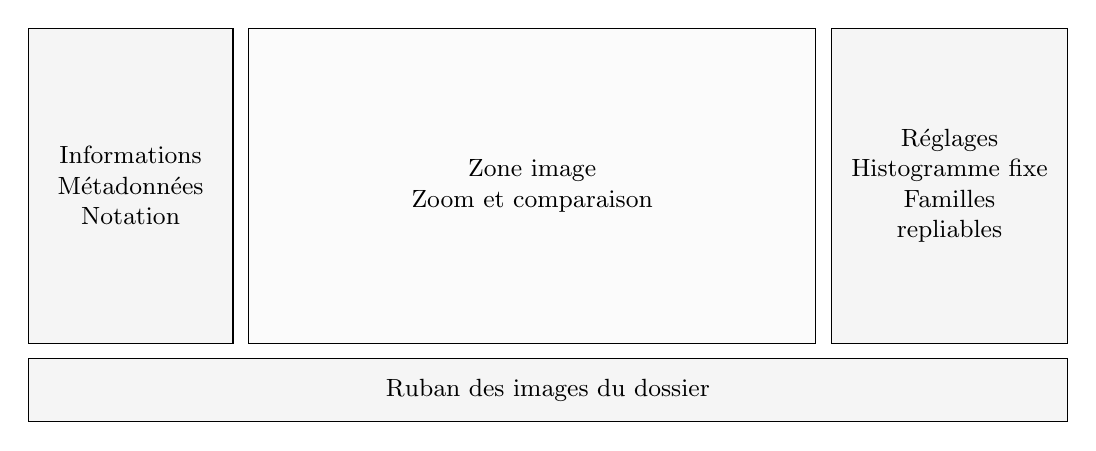
\begin{tikzpicture}[x=1cm,y=1cm,every node/.style={font=\small,align=center}]
\draw[fill=gray!8] (0,1) rectangle (2.6,5);
\draw[fill=gray!3] (2.8,1) rectangle (10,5);
\draw[fill=gray!8] (10.2,1) rectangle (13.2,5);
\draw[fill=gray!8] (0,0) rectangle (13.2,0.8);
\node at (1.3,3) {Informations\\Métadonnées\\Notation};
\node at (6.4,3) {Zone image\\Zoom et comparaison};
\node at (11.7,3) {Réglages\\Histogramme fixe\\Familles\\repliables};
\node at (6.6,0.4) {Ruban des images du dossier};
\end{tikzpicture}
\end{center}
Ce schéma représente l’organisation de l’interface, pas une capture d’écran.
Le menu \emph{Affichage} permet de masquer les informations, l’histogramme
ou le ruban. Un clic sur l’en-tête d’une famille déplie ou replie ses réglages.
Le repliement ne remet pas les valeurs à zéro.

\section{Un premier développement simple}
\begin{enumerate}
\item Ouvrir une photo et attendre la fin du traitement.
\item Vérifier son profil, puis ajuster l’exposition dans \emph{Lumière}.
\item Comparer l’original et l’état courant ; vérifier les détails au zoom.
\item Ajuster la couleur, puis le bruit et la netteté si nécessaire.
\item Exporter une copie avec le récapitulatif décrit au chapitre~\ref{chap:export}.
\end{enumerate}

\section{Comprendre les traitements en cours}
Un badge apparaît sur la zone image lorsqu’un traitement dure suffisamment
longtemps. Un aperçu boîtier peut précéder le développement IPR : il est alors
identifié explicitement. La description RAW / Profil reste stable pendant
un simple calcul de retouche pour ne pas déplacer les commandes.
Le message au bas de la fenêtre apporte les détails et les erreurs.

\attention{Le badge est générique, pas une jauge en pourcentage. Il n’expose
pas encore séparément toutes les étapes du moteur. L’absence de badge ne
remplace pas la lecture d’un éventuel message d’erreur.}

\section{Retouches et sauvegarde}
Les réglages sont mémorisés dans un fichier compagnon \chemin{.ipr}, à côté
de la source : par exemple \chemin{photo.CR3.ipr}. Le fichier source n’est
pas réécrit par ces retouches. Garder le compagnon avec l’image lors d’un
déplacement ou d’une sauvegarde ; vérifier les droits d’écriture du dossier.
Le stockage est automatique et différé : attendre les traitements et vérifier
les éventuels avertissements de sauvegarde avant de quitter.

\attention{Le fichier compagnon n’est ni une copie de la photo ni un export.
Les préférences de l’interface sont, elles, stockées dans un INI distinct.}
